\documentclass{standalone}
\usepackage{tikz}
\usetikzlibrary{patterns}
\usepackage{pgfplots}
\begin{document}%
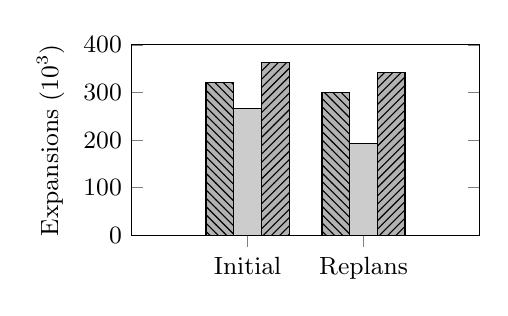
\begin{tikzpicture}[font=\small]

% this stats are currently manually computed
% from results of experiment: Makefile.incbi-road-ne

\begin{axis}[
   ybar=0pt,
   %bar width=0.20cm,
   enlarge x limits=1.0,
   width=6cm, height=4cm,
   ymin=0,
   ylabel={Expansions ($10^3$)},
   xlabel near ticks,
   ylabel near ticks,
   xtick=data,
   symbolic x coords={Initial,Replans},
   xtick pos=left,
   ]

% lpastar
\addplot+[draw=black,fill=black!30,postaction={pattern=north west lines}]
coordinates
{
   (Initial,321.71094)
   (Replans,300.314597778)
};

% incbi
\addplot+[draw=black,fill=black!20]
coordinates
{
   (Initial,267.04973)
   (Replans,193.429478889)
};

% rlpastar
\addplot+[draw=black,fill=black!30,postaction={pattern=north east lines}]
coordinates
{
   (Initial,363.66522)
   (Replans,341.62907)
};

\end{axis}

\end{tikzpicture}%
\end{document}
